\documentclass{article}
\usepackage{listings}
\usepackage{xcolor}
\usepackage{graphicx}

\title{File Transfer System Design and Implementation}
\author{Vu Hai Thien Long (22BI13268) \\ Luu Linh Ly (22BI13269) \\ Nguyen Duc Duy (22BI13120) \\ Le Viet Hoang Lam (22BI13235) \\ Nguyen Ngoc Nhi (22BI13351)}
\date{28 November 2024}

\lstdefinestyle{mypython}{
    language=Python,
    backgroundcolor=\color{white},   % background color
    basicstyle=\ttfamily\footnotesize, % font style and size
    keywordstyle=\color{blue},         % keywords in blue
    commentstyle=\color{gray},         % comments in gray
    stringstyle=\color{red},           % strings in red
    numberstyle=\tiny\color{gray},    % line numbers in gray
    numbers=left,                     % show line numbers on the left
    stepnumber=1,                     % step between line numbers
    numbersep=10pt,                   % distance between line numbers and code
    frame=single,                     % frame around code
    rulecolor=\color{black},          % color of frame
    breaklines=true,                  % line breaks
    breakatwhitespace=true,           % break lines at whitespaces
    showstringspaces=false,           % hide spaces in strings
    captionpos=b,                     % caption position at the bottom
}

\begin{document}

\maketitle



\section{Design of the Protocol}

In this file transfer system, the client sends a file to the server over a TCP connection. The communication protocol is designed to handle multiple clients, allow file transfer in chunks, and allow the server to handle requests until it is explicitly shut down.

\subsection{Communication Protocol Design}
\begin{itemize}
    \item \textbf{Client to Server Communication}:
    \begin{itemize}
        \item \textbf{Client Request}: The client establishes a TCP connection to the server by connecting to the server’s IP address and port number.
        \item \textbf{File Transfer}: Once the connection is established, the client opens the file to be sent and sends the file data in 1024-byte chunks to the server. The transfer continues until the entire file is sent.
        \item \textbf{Server Acknowledgment}: Once the file transfer is complete, the server stores the received data in a file named \texttt{received\_file.txt}. It does not send an acknowledgment back to the client explicitly.
        \item \textbf{Server Shutdown Command}: The server listens for a \texttt{"stop"} command to shut down. This is handled through the \texttt{stop\_server\_event} event, which, when set, causes the server to exit.
    \end{itemize}
    \item \textbf{File Transfer Process Flow}:
    \begin{enumerate}
        \item \textbf{Client Side}:
        \begin{itemize}
            \item The client connects to the server.
            \item The client sends the file in chunks.
            \item Once the file is fully transferred, the client terminates the connection.
        \end{itemize}
        \item \textbf{Server Side}:
        \begin{itemize}
            \item The server listens for incoming connections and accepts a file transfer.
            \item The server writes the received chunks to a file and waits for the next connection.
            \item The server continues to accept new client connections until the \texttt{"stop"} command is entered.
        \end{itemize}
    \end{enumerate}
\end{itemize}

\section{System Flow Diagram}

To better visualize how the system works, below is our system flow diagram.


\begin{figure}[h!]
    \centering
    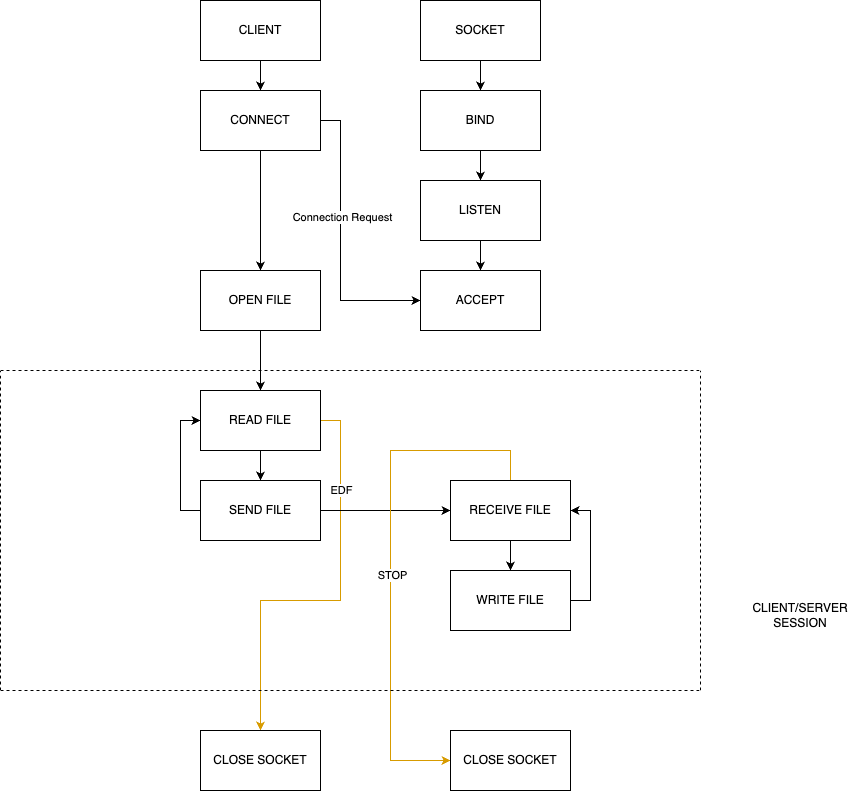
\includegraphics[width=1\textwidth]{flow.png}
    \caption{File Transfer Process Flow}
    \label{fig:flow}
\end{figure}

\subsection{Explanation of Flow Diagram}
\begin{itemize}
    \item \textbf{Client}: Connects to the server and sends the file in 1024-byte chunks.
    \item \textbf{Server}: Receives the data, writes it to a file, and continues listening for new client connections.
    \item The process continues until the server receives the "stop" command.
\end{itemize}


\section{File Transfer Implementation}

The file transfer system involves the following key components:
\begin{itemize}
    \item \textbf{Socket Setup}: Both the client and server establish a socket connection for communication.
    \item \textbf{File Reading and Sending}: The client reads the file in chunks and sends it to the server.
    \item \textbf{File Receiving and Writing}: The server receives the file data in chunks and writes it to disk.
\end{itemize}

\subsection{Client Code Snippet}

\begin{lstlisting}[style=mypython]
import socket

def send_file(file_path, host='127.0.0.1', port=65432):
    # Create a socket
    with socket.socket(socket.AF_INET, socket.SOCK_STREAM) as client_socket:
        client_socket.connect((host, port))
        print(f"Connected to server at {host}:{port}")
        
        # Open and send the file
        with open(file_path, "rb") as file:
            while chunk := file.read(1024):  # Read file in chunks
                client_socket.sendall(chunk)
        print(f"File '{file_path}' sent to the server.")

if __name__ == "__main__":
    file_path = input("Enter the path to the file you want to send: ")
    send_file(file_path)
\end{lstlisting}

\subsection{Server Code Snippet}

\begin{lstlisting}[style=mypython]
import socket
import threading

def start_server(host='127.0.0.1', port=65432):
    def handle_clients():
        with socket.socket(socket.AF_INET, socket.SOCK_STREAM) as server_socket:
            server_socket.bind((host, port))
            server_socket.listen()
            print(f"Server listening on {host}:{port}")
            
            while not stop_server_event.is_set():  # Run until stop_server_event is triggered
                try:
                    conn, addr = server_socket.accept()
                    with conn:
                        print(f"Connected by {addr}")
                        with open("received_file.txt", "wb") as file:
                            while True:
                                data = conn.recv(1024)
                                if not data:
                                    break
                                file.write(data)
                        print("File received and saved as 'received_file.txt'")
                except socket.error:
                    break
    
    # Start a thread to handle client connections
    threading.Thread(target=handle_clients, daemon=True).start()
    
    # Wait for the "stop" command
    while True:
        command = input("Type 'stop' to shut down the server: ").strip().lower()
        if command == 'stop':
            stop_server_event.set()
            print("Shutting down the server...")
            break

if __name__ == "__main__":
    stop_server_event = threading.Event()  # Event to signal server shutdown
    start_server()
\end{lstlisting}





\section{Conclusion}

This system is a simple and effective way to transfer files over a network using TCP sockets. The server handles multiple clients by running in a separate thread, and the client can send files in chunks to ensure efficient transfer. The server is designed to continue running until the "stop" command is given, making it a robust solution for ongoing file transfers.

\end{document}
